\documentclass{scrbook}

%!TEX root = thesis.tex

% Set german to default language and load english as well
\usepackage[ngerman,english]{babel}

% Set UTF8 as input encoding
\usepackage[utf8]{inputenc}

% Set T1 as font encoding
\usepackage[T1]{fontenc}
% Load a slightly more modern font
\usepackage{lmodern}
% Use the symbol collection textcomp, which is needed by listings.
\usepackage{textcomp}
% Load a better font for monospace.
\usepackage{courier}

% Set some options regarding the document layout. See KOMA guide
\KOMAoptions{%
  paper=a4,
  fontsize=12pt,
  parskip=half,
  headings=normal,
  BCOR=1cm,
  headsepline,
  DIV=12}

% do not align bottom of pages
\raggedbottom

% set style of captions
\setcapindent{0pt} % do not indent second line of captions
\setkomafont{caption}{\small}
\setkomafont{captionlabel}{\bfseries}
\setcapwidth[c]{0.9\textwidth}

% set the style of the bibliography
\bibliographystyle{alphadin}

% load extended tabulars used in the list of abbreviation
\usepackage{tabularx}

% load the color package and enable colored tables
\usepackage[table]{xcolor}

% define new environment for zebra tables
\newcommand{\mainrowcolors}{\rowcolors{1}{maincolor!25}{maincolor!5}}
\newenvironment{zebratabular}{\mainrowcolors\begin{tabular}}{\end{tabular}}
\newcommand{\setrownumber}[1]{\global\rownum#1\relax}
\newcommand{\headerrow}{\rowcolor{maincolor!50}\setrownumber1}

% add main color to section headers
\addtokomafont{chapter}{\color{maincolor}}
\addtokomafont{section}{\color{maincolor}}
\addtokomafont{subsection}{\color{maincolor}}
\addtokomafont{subsubsection}{\color{maincolor}}
\addtokomafont{paragraph}{\color{maincolor}}

% do not print numbers next to each formula
\usepackage{mathtools}
\mathtoolsset{showonlyrefs}
% left align formulas
\makeatletter
\@fleqntrue\let\mathindent\@mathmargin \@mathmargin=\leftmargini
\makeatother

% Allow page breaks in align environments
\allowdisplaybreaks

% header and footer
\usepackage{scrpage2}
\pagestyle{scrheadings}
\setkomafont{pagenumber}{\normalfont\sffamily\color{maincolor}}
\setkomafont{pageheadfoot}{\normalfont\sffamily}
\setheadsepline{0.5pt}[\color{maincolor}]

% German guillemets quotes
\usepackage[german=guillemets]{csquotes}

% load TikZ to draw diagrams
\usepackage{tikz}

% load additional libraries for TikZ
\usetikzlibrary{%
  automata,%
  positioning,%
}

% set some default options for TikZ -- in this case for automata
\tikzset{
  every state/.style={
    draw=maincolor,
    thick,
    fill=maincolor!18,
    minimum size=0pt
  }
}

% load listings package to typeset sourcecode
\usepackage{listings}

% set some options for the listings package
\lstset{%
  upquote=true,%
  showstringspaces=false,%
  basicstyle=\ttfamily,%
  keywordstyle=\color{keywordcolor}\slshape,%
  commentstyle=\color{commentcolor}\itshape,%
  stringstyle=\color{stringcolor}}

% enable german umlauts in listings
\lstset{
  literate={ö}{{\"o}}1
           {Ö}{{\"O}}1
           {ä}{{\"a}}1
           {Ä}{{\"A}}1
           {ü}{{\"u}}1
           {Ü}{{\"U}}1
           {ß}{{\ss}}1
}

% define style for pseudo code
\lstdefinestyle{pseudo}{language={},%
  basicstyle=\normalfont,%
  morecomment=[l]{//},%
  morekeywords={for,to,while,do,if,then,else},%
  mathescape=true,%
  columns=fullflexible}

% load the AMS math library to typeset formulas
\usepackage{amsmath}
\usepackage{amsthm}
\usepackage{thmtools}
\usepackage{amssymb}

% load the paralist library to use compactitem and compactenum environment
\usepackage{paralist}

% load varioref and hyperref to create nicer references using vref
\usepackage[english]{varioref}
\PassOptionsToPackage{hyphens}{url} % allow line break at hyphens in URLs
\usepackage{hyperref}

% setup hyperref
\hypersetup{breaklinks=true,
            pdfborder={0 0 0},
            ngerman,
            pdfhighlight={/N},
            pdfdisplaydoctitle=true}

% Fix bugs in some package, e.g. listings and hyperref
\usepackage{scrhack}

%!TEX root = thesis.tex

% Use this file to define some macros you need in your thesis. A macro is a short command that inserts some mathematical symbols or texts you do not want to retype each time you need some. I recommend to use as many macros as possible, because you are able to change them later. For example if you use the same macro each time you need to give the formal semantics of an expression you can easily change the appearance of these brackets by updating the macro later on.

% Set of natural numbers
\newcommand{\N}{\mathbb{N}}

% The default epsilon does not look very nice
\let\epsilon\varepsilon

% If you need to use mathematical expressins like an epsilon in the section titles of your thesis you will end up with warnings that these special symbols cannot be included in the PDF favorites. The following macro uses the mathematical symbol during the text of the thesis and the string "Epsilon" in the PDF favorites.
\newcommand{\pdfepsilon}{\texorpdfstring{$\epsilon$}{Epsilon}}


% Set title and author used in the PDF meta data
\hypersetup{
  pdftitle={Don't Copy That Floppy},
  pdfauthor={Yara Eid, Jonas Lamperti}
}

% Depending on which of the following two color schemes you import your thesis will be in color or grayscale. I recommend to generate a colored version as a PDF and a grayscale version for printing.

%!TEX root = thesis.tex

% define color of example university
\xdefinecolor{exampleuniversity}{rgb}{1, 0.5, 0}

\colorlet{maincolor}{exampleuniversity}

\colorlet{stringcolor}{green!60!black}
\colorlet{commentcolor}{black!50}
\colorlet{keywordcolor}{maincolor!80!black}

\newcommand{\imagesuffix}{-color}
%%!TEX root = thesis.tex

\colorlet{maincolor}{black}

\colorlet{stringcolor}{black}
\colorlet{commentcolor}{black!50}
\colorlet{keywordcolor}{black}

\newcommand{\imagesuffix}{-gray}

\newcommand{\duedate}{13. Dezember 2016}

\begin{document}
  \frontmatter
  %!TEX root = thesis.tex

\begin{titlepage}
  \thispagestyle{empty}

  \vskip1cm

  \pgfimage[height=2.5cm]{Logo_Uni_Luebeck_300dpi.png}
  
  \vskip2.5cm
  
  \LARGE
  
  \textbf{\sffamily\color{maincolor}Don't Copy That Floppy}

  \textit{Don't Copy That Floppy}

  \normalfont\normalsize

  \vskip2em
  
  \textbf{\sffamily\color{maincolor}Bachelor Thesis}

  within the context of the course \\
  \textbf{\sffamily\color{maincolor}Tools for scientific workings} \\
  at the Universität zu Lübeck

  \vskip1em

  by \\
  \textbf{\sffamily\color{maincolor}Yara Eid, Jonas Lamperti}

  \vskip1em
  
  supervised by \\
  \textbf{\sffamily\color{maincolor}Who (M.D.)}

  \vskip1em

  \vfill

  Lübeck, \duedate
\end{titlepage}

  %!TEX root = thesis.tex

\cleardoublepage
\thispagestyle{plain}
\vspace*{\fill}

\section*{Declaration of Authenticity}
I declare that all material presented in this paper is my own work or fully and
specifically acknowledged wherever adapted from other sources.
I understand that if at any time it is shown that we have significantly misrepresented
material presented here, any degree or credits awarded to us on the basis of that
material may be revoked.
I declare that all statements and information contained herein are true, correct and
accurate to the best of my knowledge and belief.

\vskip2cm

\rule{5cm}{0.4pt}\\
(Yara Eid, Jonas Lamperti)\\
Lübeck, den \duedate

  %!TEX root = thesis.tex

\cleardoublepage
\thispagestyle{plain}

\pdfbookmark{Abstract}{abstract}
\paragraph{Abstract}
Don't Copy That Floppy was an anti-copyright infringement campaign run by the Software Publishers Association (SPA) beginning in 1992.\cite{Edg03} The video for the campaign, starring M. E. Hart as "MC Double Def DP," was filmed at Cardozo High School in Washington, D.C. and produced by cooperation between the SPA, the Educational Section Anti-Piracy Committee, and the Copyright Protection Fund, in association with Vilardi Films. The groups distributed the film for general viewing through VHS tapes that were mailed to schools. In later years, the film became a viral video sensation through websites such as YouTube, where the official page has had over 1,000,000 views as of December 2013.

In May 2009, the Software and Information Industry Association (formed in 1999 when the Software Publishers Association merged with the Information Industry Association) released the trailer for a follow-up to Don't Copy That Floppy, called Don't Copy That 2, released on September 9, 2009. The sequel features MC Double Def DP as he continues his crusade against "piracy" in the digital age.

\begin{figure}

\includegraphics{220px-Dontcopythatfloppy3.jpg}
\caption{Screenshot from ad showing Corey and Jenny playing a video game.}
\label{fig:kids}
\end{figure}

\cleardoublepage
\thispagestyle{plain}

\foreignlanguage{german}{%
\pdfbookmark{Kurzfassung}{kurzfassung}
\paragraph{Kurzfassung} 
 ''Don't Copy That Floppy'' war eine Kampagne gegen Urheberrechtsverletzungen der Software Publishers Association (SPA), welche 1992 begann. Das Video zur Kmpagne, mit M. E. Hart in der Hauptrolle als ''MC Double Def DP'', wurde in der Cardozo High School in Washington, D.C.  gefilmt. Es wurde produziert von einer Kooperation zwischen SPA, dem Educational Section Anti-Piracy Committee, dem Copyright Protection Fund, in Zusammenarbeit mit Vilardi Films. The gruppen verteilten den Film zur Vorführung auf VHS-Kassetten, welche an Schulen verschickt wurden. Einige Jahre später wurde der Film zum viralen Hit auf Video-Streming Seiten wie Youtube, wo die offizielle Seite im Dezember 2013 über 1 Mio. Aufrufe hatte. \\ 
  Im Mai 2009 veröffentliche die the Software and Information Industry Association (entstanden 1999, als sich die Software Publishers Association mit der Information Industry Association zusammenschloss) einen Trailer für einen Nachfolger zu Don't Copy That Floppy, Don't Copy That 2, welcher am 9.September 2009 erschien. Der Nachfolger zeigt, wie MD Couble Pref seinen Kreuzzug gegen Internet-Piraterie im digitalen Zeitalter fortsetzt.
}

  \cleardoublepage
  \phantomsection
  \pdfbookmark{Inhaltsverzeichnis}{tableofcontents}
  \markboth{Inhaltsverzeichnis}{}
  \tableofcontents

  \mainmatter
  %!TEX root = thesis.tex

\chapter{Synopsis}

\begin{figure}
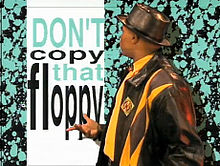
\includegraphics{220px-Dontcopythatfloppy.jpg}
\caption{The ''Disk Protector'' showing the title of the campaign during the rap portion of the video.}
\label{fig:disk_protector}
\end{figure}

Two teenagers, Jenny (played by Marja Allen) and Corey (played by Jimmy Todd), are playing a game on a classroom computer. Corey is exuberantly pushing keys to show the viewer that he is heavily immersed in the game action; Jenny is beating him. Frustrated, he asks for a rematch, but she has an upcoming class and must leave. He decides he will copy the game so that he can play it at home. Upon inserting his blank floppy disk into the Apple Macintosh LC a video pops up on the computer. This video is of a rapper named MC Double Def DP the ''Disk Protector.''

The point of the video is the message that copyright infringement of software will cause the computer and video game industry to lose profit, resulting in halted production of further computer games. \cite{onpi} (The games the video chooses as examples—The Oregon Trail, Tetris, and the Where in the World is Carmen Sandiego? series—were among the most successful and bestselling games of the late-1980s to mid-1990s.)

The rap video portion is interspersed with interviews of artists, writers, programmers and a lawyer. These people are the staff responsible for design of an early version of the game Neverwinter Nights (then an America Online MMORPG) and allows them to explain the issue in greater detail:
\begin{itemize}

    \item Craig Dykstra—America Online—Manager Developer Support
    \item Dave Butler—America Online—Director Platform Software Development
    \item Janet Hunter—America Online—Senior Systems Analyst
    \item Ilene Rosenthal—Software Publishers Association—Attorney
    
\end{itemize}

They explain how games are made, indicating that creating a game can involve 20 to 30 people integrating the various parts, and working on documentation, technical support, and marketing. The point they try to raise is that if sales are low, the authors may decide that the game is unpopular and stop making it.

At the end of the video the DP fades away, leaving Corey and Jenny to decide for themselves whether they will copy the game—they decide against it. Corey, who has some money left over from his summer job, decides that he will buy the game. Jenny agrees and jokes that Corey's game will even come with a manual.

The Wall Street Journal has stated that the film's aesthetic is similar to the TV program Saved By the Bell. It has also highlighted it as an example of classic bubblegum hip-hop with long-run staying power.
\section{Structure of the Thesis}

Apart from the Sysnopsis this Thesis is divided into the following parts:
\begin{description}
  \item[\ref{Criticism}] describes the Reception by the press.
  \item[\ref{popularity_online}] describes the rise of the Video to a meme.
  \item[\ref{sequel}] descibes the Sequel to the video and it's reception.
\end{description}


  %!TEX root = thesis.tex

\chapter{Criticism}
\label{Criticism}

The major criticism of the campaign came from educators and the press, who criticized the campaign for only promoting one point of view, instead of a broader scope of the issue of copyright online. That point of view, they argued, was biased because it benefited a specific group (the software publishing industry), and failed to present alternative views such as the Free Software movement. \cite{piracy}
  %!TEX root = thesis.tex

\chapter{Popularity Online}
\label{popularity_online}In the late 2000s, the popularity of the video was revived, but this time as a meme. Since the creators have always allowed non-commercial copying of the film, it became a viral video after video-sharing sites such as Google Video and YouTube went online in the mid-2000s. The video first gained popularity on the site YTMND in 2004 and then gained (and re-gained) widespread YouTube popularity in 2005, 2006, and 2008, sparking user-generated remixes and parodies, and is now considered a popular internet meme.
  %!TEX root = thesis.tex

\chapter{Sequel}
\label{sequel}
In May 2009, the Software and Information Industry Association (SIIA) released the trailer for a follow-up to the original 1992 video, which premiered on September 9, 2009. Don't Copy That 2 features M. E. Hart reprising his role as ''MC Double Def DP''. The trailer shows armed SWAT police raiding homes and arresting the mothers of would-be pirates. The SIIA website says that ''Antipiracy hero MC Double Def DP will return to drop some knowledge on would-be pirates in the sequel to 1992's 'Don't Copy That Floppy.'.''

\section{Criticism}
Don't Copy That 2 has received over 517,000 views on YouTube as of September 14, 2015. Since its release it has been criticized by the press for being out of date, referencing material like the Doom series and Klingon that the current target audience (mostly teenagers) may not be familiar with. The sequel was also heavily criticized in the press for misrepresenting the way copyright law is enforced, what types of copying were actually considered ''criminal'' enough to prompt punishment, and what punishment actually looked like.

  \appendix

  %!TEX root = thesis.tex

\chapter{Appendix}

This section contains information that is not directly part of the thesis.


  \backmatter

  \cleardoublepage
  \phantomsection
  \pdfbookmark{List of Figures}{listoffigures}
  \listoffigures


  %!TEX root = thesis.tex

\cleardoublepage
\phantomsection
\pdfbookmark{abbreviations}{abbreviations}
\chapter*{List of Abreviations}
\label{section-abbrevs}

\begin{tabularx}{\textwidth}{lX}
  ABA & alternierender Büchi-Automat, engl. \emph{a}lternating \emph{B}üchi \emph{a}utomaton\\
  AFA & alternierender endlicher Automat, engl. \emph{a}lternating \emph{f}inite \emph{a}utomaton\\
  BA & Büchi-Automat, engl. \emph{B}üchi \emph{a}utomaton\\
  BNF & Normalform kontextfreier Grammatiken, engl. \emph{B}ackus--\emph{N}aur \emph{f}orm\\
  DFA & endlicher Automat, engl. \emph{d}eterministic \emph{f}inite \emph{a}utomaton\\
  SPA & Software Publishers Association
\end{tabularx}


  \cleardoublepage
  \phantomsection
  \pdfbookmark{Bibliography}{bibliography}
  \bibliography{literature}
\end{document}
